\documentclass[twoside]{article}
\usepackage[accepted]{aistats2e}
\usepackage[latin2]{inputenc}
\usepackage{amsmath}
\usepackage{amssymb}
\usepackage{multirow}
\usepackage{microtype}
\usepackage[round]{natbib}
\usepackage{bm}
\usepackage{algorithmic}
\usepackage[
    pdfstartview={FitH},
    bookmarks=true,
    bookmarksnumbered=true,
    bookmarksopen=true,
    bookmarksopenlevel=\maxdimen,
    pdfborder={0 0 0},
    colorlinks=true,
    linkcolor = black,
    citecolor=black,
    urlcolor=black,
    filecolor=black,
    pdfauthor={Simon Lacoste-Julien, Ferenc Husz�r, Zoubin Ghahramani},
    pdftitle={Approximate inference for the loss-calibrated Bayesian},
    pdfdisplaydoctitle=true
]{hyperref}
\usepackage[pdftex]{graphicx}
\usepackage{tikz}
\usepackage{atbeginend}
\usetikzlibrary{arrows,shapes,backgrounds}

\newcommand{\secref}[1]{Sec.~\ref{#1}}
\newcommand{\tableref}[1]{Table~\ref{#1}}
\newcommand{\figref}[1]{Fig.~\ref{#1}}
\newcommand{\chapref}[1]{Ch.~\ref{#1}}
\newcommand{\appref}[1]{Appendix~\ref{#1}}
\newcommand{\dataset}{\mathcal{D}}
\newcommand{\prob}[1]{\boldsymbol{\mathbb{#1}}}
\newcommand{\Var}{\mathbb{V}\!\textnormal{ar}}
\newcommand{\fix}[1]{$^\text{\textcolor{red}{?}}$\marginpar[\raggedleft\parbox{2.5cm}{\raggedleft \tiny{#1}}]{\parbox{2.5cm}{\tiny{#1}}}}
\newcommand{\new}{\marginpar{NEW}}
\newcommand{\argmin}[1]{\underset{#1}{\arg\min\:}}
\newcommand{\argmax}[1]{\underset{#1}{\arg\max\:}}


%% space saving tricks!!
\renewcommand{\baselinestretch}{0.98} % super powerful!
%\addtolength{\textfloatsep}{-5mm} %problems with footnotes...

\newenvironment{shrinkeq}[1]
{ \bgroup
  \addtolength\abovedisplayshortskip{#1}
  \addtolength\abovedisplayskip{#1}
  \addtolength\belowdisplayshortskip{#1}
  \addtolength\belowdisplayskip{#1}}
{\egroup\ignorespacesafterend}

\AfterBegin{itemize}{\addtolength{\itemsep}{-0.5\baselineskip}}

%\raggedbottom % this is to see where extra space is at the bottomm...

\begin{document}

\twocolumn[
\aistatstitle{Approximate inference for the loss-calibrated Bayesian}

%\aistatsauthor{ Anonymous Author(s) }
\aistatsauthor{ Simon Lacoste-Julien \And Ferenc Husz\'{a}r \And Zoubin Ghahramani }

\aistatsaddress{ University of Cambridge \And University of Cambridge \And  University of Cambridge }
% SUPER UGLY: \aistatsaddress{Computational and Biological Learning Laboratory, Department of Engineering, University of Cambridge}

%\aistatsaddress{ Top Secret Institution(s) }
]

\begin{abstract}
We consider the problem of approximate inference in the context of Bayesian decision theory. Traditional approaches focus on approximating general properties of the posterior, ignoring the decision task -- and associated losses -- for which the posterior could be used. We argue that this can be suboptimal and propose instead to \emph{loss-calibrate} the approximate inference methods with respect to the decision task at hand. We present a general framework rooted in Bayesian decision theory to analyze approximate inference from the perspective of losses, opening up several research directions. As a first loss-calibrated approximate inference attempt, we propose an EM-like algorithm on the Bayesian posterior risk and show how it can improve a standard approach to Gaussian process classification when losses are asymmetric.
\end{abstract}

\section{INTRODUCTION}

%In the first session of the last Valencia International Meetings on Bayesian Statistics, Simon French\footnote{Who interestingly was one of the only two attendees who said having participated in all 9 Valencia meetings.} %OPTIONAL!
%surveyed the rich history of Bayesian statistics and highlighted the need to go back to study the interplay between \emph{foundations} and \emph{computation}. This paper endeavors to do just that. % pompous? Less pompous: This paper is our first attempt for that.
%The Bayesian paradigm is often theoretically motivated in terms of arguments of coherence in the context of decision making. We will thus focus on statistical Bayesian decision theory as
%
%[Intro from Snowbird abstract -- to change!] \\
%- Bayesian paradigm from Bayesian decision theory \\
%- coherent framework and optimal if do exact inference \\
%- but not for approximate inference; we want to correct that and explore it \\
%- Contributions? \\
Bayesian methods have enjoyed a surge of popularity in machine learning over the last decade. Even though it is sometimes overlooked, the main theoretical motivations for the Bayesian paradigm are rooted in Bayesian decision theory~\citep{berger85decision}, which provides a well-defined theoretical framework for rational decision making under uncertainty about a hidden parameter $\theta$. The ingredients of Bayesian decision theory are an observation model $p(\dataset|\theta)$, a prior distribution $p(\theta)$, and a loss $L(\theta,a)$ for an action $a\in\mathcal{A}$. In this framework, the optimal action is chosen by minimizing its expected loss over the posterior $p(\theta|\dataset)$. The independence of the posterior from the loss motivates the common practice of breaking decision making into two independent sub-problems: \emph{inference}, whereby the posterior $p(\theta|\dataset)$ is computed irrespectively of the loss; and then \emph{decision}, whereby an action is chosen to minimize its expected loss over our posterior belief.

In practically interesting Bayesian models, however, the posterior is often computationally intractable and therefore one has to resort to approximate inference techniques, such as variational methods or Markov chain Monte Carlo. Most approaches to approximate inference ignore the decision theoretic loss and try to approximate the posterior based on its general features, such as matching its mode or higher order moments. While this is probably a reasonable approach for the simple losses usually considered or when the loss is unknown, they might fail to work well with asymmetric, non-trivial losses that appear in modern applications in machine learning.

The main message of the present paper is that when inference is carried out only approximately, treating (approximate) inference and decision making independently can lead to suboptimal decisions for a fixed loss under consideration. We thus investigate whether one can ``calibrate'' the approximate inference algorithm to a fixed loss, and propose an analysis framework to analyze this situation. We note that a related philosophy has already been applied in the frequentist discriminative machine learning literature, as for example with the use of \emph{surrogate loss functions} \citep{bartlett06risk,steinwart08svm}. In contrast, we focus in this paper on the pure subjectivist Bayesian viewpoint as we are not yet aware of the existence of such an investigation in this case. The contributions of the present paper can be summarized as follows:
\begin{enumerate}
	\item In \secref{s:setup}, we propose a general approximate inference framework based on Bayesian decision theory to guide our analysis. The framework naturally gives rise to a divergence between distributions that can be seen as a loss-calibrated generalization of the Kullback-Leibler divergence for general losses. We focus in this paper on the application of the framework to the predictive setting that is relevant to supervised machine learning.
	\item In \secref{s:EM-alg}, we present an algorithmic template to derive loss-calibrated approximate inference algorithms for different losses by applying the variational Expectation-Maximization algorithm on the Bayesian posterior risk.
	\item In \secref{s:examples}, we investigate our approximation framework on the concrete setup of supervised learning. We apply the loss-calibrated EM algorithm to a Gaussian process classification model and analyze its performance in terms of the loss-calibrated framework. Our proof-of-concept experiments indicate that it improves over a loss-insensitive approximate inference alternative and that the advantage of loss-calibration is more prominent when misclassification losses are asymmetric.
\end{enumerate}

\section{BAYESIAN DECISION THEORY} \label{s:setup}

We use Bayesian statistical decision theory as the basis of our analysis (see Ch.~2 of~\citet{robert01choice} or Ch.~1 of~\citet{berger85decision} for example). We review here its main ingredients:
\vspace{-.3cm}
\begin{itemize}
  \item a (statistical) loss $L(\theta,a)$ which gives the cost of taking action $a \in \mathcal{A}$ when the world state is $\theta \in \Theta$; %\footnote{Note that $\theta$ is not assumed to be finite dimensional; in the most general setting, it could fully specify an arbitrary distribution over $\mathcal{O}$.};
  \item an observation model $p(\dataset|\theta)$ which gives the probability of observing $\dataset \in \mathcal{O}$ assuming that the world state is $\theta$;
  \item a prior belief $p(\theta)$ over world states.
\end{itemize}
%\vspace{-.3cm}
The loss $L$ describes the decision task that we are interested in, whereas the observation model and the prior represent our beliefs about the world. Given these, the Bayesian evaluation metric for a possible action $a$ after observing $\dataset$ is the \emph{expected posterior loss} (also called the \emph{posterior risk}~\citep{schervish95theory}): $\mathcal{R}_{p_\dataset}(a) \doteq \int_\Theta L(\theta, a) \, p(\theta|\dataset) d\theta$, and so the (Bayes) optimal action $a_{p_\dataset}$ is the one that minimizes $\mathcal{R}_{p_\dataset}$.
%\footnote{This action exists under suitable regularity conditions. For the sake of clarity of presentation, we will not cover such rigorous details in this paper. Amongst others, we will write general integrals without specifying the base measure (and so integrals could also be sums). We will also assume w.\,l.\,o.\,g.\ that $L(\theta,a) \geq 0$.}.
%% Maybe some words about the powerful machine learning convention of p(\theta) being different than p(x)...?
%%THE FOLLOWING IS OPTIONAL:
%(I mention the frequentist treatment because most of statistical decision theory is studied from a frequentist perspective -- so Bayesians are less familiar with it [e.g. Andrew Gelman who thought of decision theory as just medical treatment applications] and frequentists will ask how it relates to their world...

%We note that the frequentist treatment of decision theory focuses instead on the \emph{frequentist risk} function of a procedure $\delta : \mathcal{O} \rightarrow \mathcal{A}$ by averaging over possible observations: $\mathcal{R}^F(\theta,\delta) \doteq \prob{E}_{\dataset \sim p(\dataset|\theta)}[L(\theta,\delta(\dataset))]$. Because this metric is a function of the \emph{unknown} $\theta$, the optimal action is unclear and one has to design principles to compare the risk functions of different procedures (e.g. minimaxity, admissibility, etc.). One natural principle is to reduce the risk function to a scalar called the \emph{Bayes risk} by taking a weighted average over all $\theta$: $r(\delta) = \int_{\Theta} \mathcal{R}^F(\theta,\delta) p(\theta) d\theta$. The Bayesian procedure $\delta(\dataset) = a_{p_\dataset}$ mentioned above has actually minimum Bayes risk (if using the prior as the weighting function; see thm. 2.3.2 of~\citet{robert01choice}) and this is one way to relate the Bayesian procedure to a frequentist analysis. We do not take this analysis route in this paper though and focus exclusively on the Bayesian treatment of \emph{conditioning} on the observation $\dataset$ (rather than averaging over possible other datasets); $\mathcal{R}_{p_\dataset}$ will thus be our evaluation metric.
%END of optional
%Moreover, we will not cover the problem of model misspecification and will take the pure subjective viewpoint where we believe our observation model and prior as best descriptions of reality. Even in this idealized treatment, we will see that traditional approach to approximate inference may be improved by loss-calibration.

\subsection{Supervised learning} \label{ss:predictive}

We now relate this abstract decision theory setup to the typical supervised learning applications of machine learning. For a prediction task, the goal is to estimate a function $h : \mathcal{X} \rightarrow \mathcal{Y}$ where the output space $\mathcal{Y}$ can be discrete (classification) or continuous (regression). We suppose that we are given a fixed cost function $\ell(y,y')$ which gives the cost of predicting $y'$ when the true output was $y$.
%%OPTIONAL:
%In the context of \emph{structured prediction} (such as machine translation where $\mathcal{X}$ are sentences in one language and $\mathcal{Y}$ are possible translations in another language), the cost $\ell(y,y')$ is highly informative about $\mathcal{Y}$ by providing a kind of measure of dissimilarity between discrete objects, in contrast to the standard 0--1 cost for classification or quadratic cost for regression.
% which is why we want to take it in consideration during learning??? -- not sure where to put...
%%END optional
We can cast this problem in the standard statistical decision theory setting by defining a suitable prediction loss for our action $a = h$, namely the standard generalization error from machine learning:
\begin{equation} \label{e:loss}
    L(\theta,h) \doteq \prob{E}_{(x,y)\sim p(x,y|\theta)} \left[ \ell \left( y, h(x) \right) \right] .
\end{equation}
For the observation model, we will assume that we are given a training set $\dataset = \{ (x_i,y_i)_{i=1}^N \}$ of labeled observations generated i.i.d.\ from $p(x,y|\theta)$. The goal of the learning algorithm is then to output a function $h$ chosen from a set of (possibly non-parametric) hypotheses $\mathcal{H}$ after looking at the (training) data $\dataset$. From the pure Bayesian point of view, the best hypothesis $h_{p_\dataset}$ is clear: it is the one that minimizes the posterior risk, i.e. $h_{p_\dataset} \doteq \arg\min_{h \in \mathcal{H}} \mathcal{R}_{p_\dataset} (h)$.
%Unfortunately, the required posterior $p_\dataset(\theta) \doteq p(\theta | \mathcal{D})$ is rarely computable in a tractable form. We now

\subsection{General approximation framework} \label{ss:app_framework}

The quantity central to the Bayesian methodology is the posterior $p_\dataset(\theta) \doteq p(\theta | \mathcal{D})$ which summarizes our uncertainty about the world. On the other hand, it is rarely computable in a tractable form, and so it is usually approximated with a tractable approximate distribution $q(\theta) \in\mathcal{Q}$. Popular approaches to this problem include sampling, variational inference -- which minimizes $KL( q \| p_\dataset)$, and expectation propagation -- which minimizes $KL( p_\dataset \| q)$ \citep{minka2001ep}. Most approximate inference approaches stop at $q$, though in the context of decision theory, we still need to \emph{act}. In practice, one usually treats the approximate $q$ as if it was the true posterior and chooses the action that minimizes what we will call the \emph{$q$-risk}:
\begin{equation} \label{e:q-risk}
    \mathcal{R}_q(h) \doteq \int_\Theta q(\theta) L(\theta,h) d\theta ,
\end{equation}
obtaining a \emph{$q$-optimal} action $h_q$:
\begin{equation}
    h_q \doteq \argmin{h \in \mathcal{H}} \mathcal{R}_q(h).
\end{equation}
In this paper, we will assume that computing exactly the $q$-optimal action $h_q$ for $q \in \mathcal{Q}$ is tractable, and focus on the problem of choosing a suitable $q$ to approximate the posterior $p_\dataset$ \emph{in order to yield a decision $h_q$ with low posterior risk $\mathcal{R}_{p_\dataset}(h_q)$}, mimicking the standard methodology but crystallizing the decision theoretic goal. Given this approach, a (usually non-unique) optimal $q \in \mathcal{Q}$ is clearly:
\begin{equation}
    q_\mathrm{opt} = \argmin{q \in \mathcal{Q}} \mathcal{R}_{p_\dataset}(h_q),
\end{equation}
though a practical algorithm might only be able to find an approximate minimizer to this quantity. In the case where $p_\dataset\in\mathcal{Q}$, $p_\dataset$ is obviously optimal according to this criterion.

We could interpret the above criterion as minimizing the following asymmetric non-negative discrepancy measure between distributions:
\begin{equation} \label{e:d_L}
    d_L(p\|q) \doteq \mathcal{R}_{p}(h_q) - \mathcal{R}_{p}(h_p).
\end{equation}
Interestingly, the Kullback-Leibler divergence $KL(p\|q)$ can be interpreted as a special case of $d_L$ for the task of posterior density estimation over $\Theta$. In this task, an action $h$ is a density over $\Theta$ and the standard density estimation statistical loss is $L(\theta,h) = -\log h(\theta)$. The $q$-risk $R_q(h)$ then becomes the cross-entropy $H(q,h)=-\int_\Theta q(\theta) \log(h(\theta)) d\theta$, and so $h_q = q$ assuming that $q \in \mathcal{H}$. Under these assumptions, we obtain that $KL(p\|q) = d_L(p\|q)$ and so as was already known in statistics, $KL(p_\dataset\|\cdot)$ appears ``loss-calibrated'' for the task of posterior density estimation in our approximation framework. But this begs the natural question of whether minimizing $d_L$ for a particular loss $L$ provides optimal performance under other losses. We will show in \secref{ss:GPR} that even in the simple Gaussian linear regression setting, minimizing the KL divergence can be suboptimal in the squared loss sense, thus motivating us to seek loss-calibrated alternatives.

\begin{figure}[bt]
\centering
\begin{tikzpicture}
	\node at (0.1in,0.1in) [anchor = south west] {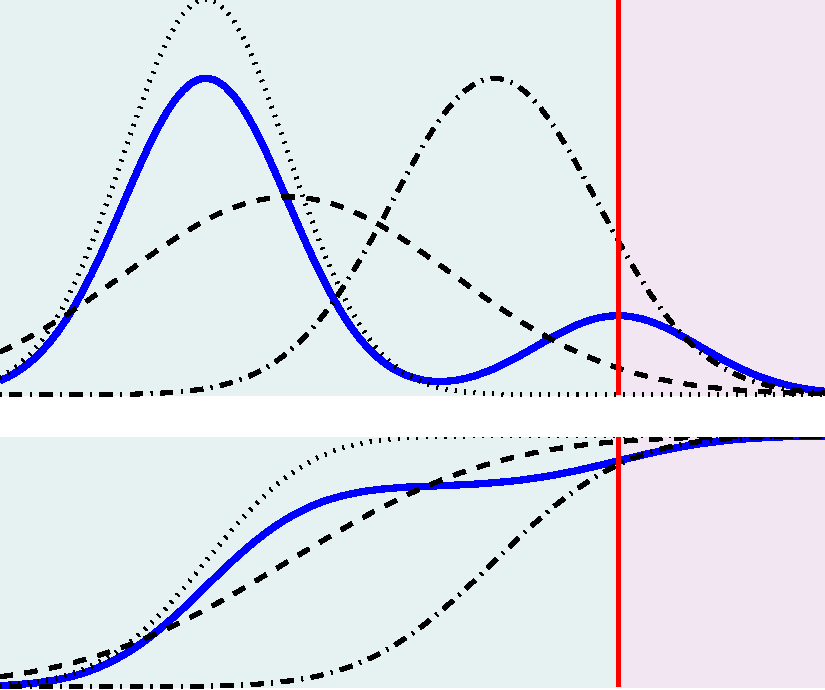
\includegraphics[width=3in]{figures/toy_figure.pdf}};
	\node at (1.6in,0in) {$\theta$ (plant temperature)};
	\node at (2.5in,0in) {$T_\mathrm{crit}$};
	\node [rotate = 90] at (0in,0.6in) {$\mathbb{P}[T<\theta]$};
	\node [rotate = 90] at (0in,2in) {$p(\theta)$};
\end{tikzpicture}
 \caption{\textbf{Top:} Real bimodal posterior \emph{(blue)} and three Gaussian approximations obtained by minimizing  $KL(q\|p)$ \emph{($q_1$, dotted)}, $KL(p\|q)$ \emph{($q_2$, dashed)} or $d_L(p\|q)$ \emph{($q_3$, dash-dotted)} in the power plant example. \textbf{Bottom:} Cumulative distribution functions for the posterior and the three approximate distributions.}  \label{fig:toy}
\end{figure}

To illustrate the difference between traditional approaches to approximate inference and the loss-calibrated framework, consider the following simple problem. Suppose that we control a nuclear power-plant which has an unknown temperature $\theta$ that we model with Bayesian inference based on some measurements $\mathcal{D}$.
The plant is in danger of over-heating, and as the operator, we can take two actions: either shut it down or keep it running. Keeping it running while the temperature is above a critical threshold $T_\mathrm{crit}$ will cause a nuclear meltdown, incurring a large loss $L(\theta>T_\mathrm{crit},\mbox{'on'})$. On the other hand, shutting down the power plant incurs a moderate loss $L(\mbox{'off'})$, irrespective of the temperature. 
%Given our posterior $p_\dataset$ and the losses, we want to compute the Bayes-optimal action that minimizes the posterior risk. 
Suppose that our current observations yielded a complicated multi-modal posterior $p_\dataset(\theta)$ (\figref{fig:toy}, solid curve) and that we thus chose to approximate it with a Gaussian. Now consider how various approaches would perform in terms of their Bayesian posterior risk. Minimizing $KL(q \| p_\dataset)$ yields candidate $q_1$ which concentrates around the largest mode, ignoring entirely the second small mode around the critical temperature (\figref{fig:toy}, dotted curve). Minimizing $KL(p_\dataset \| q)$ gives a more global approximation: $q_2$ matches moments of the posterior, but still underestimates the probability of the temperature being above $T_\mathrm{crit}$, thereby leading to a suboptimal decision (\figref{fig:toy}, dashed curve). $q_3$ is one of the minimizers of $d_L(p_\dataset \| q)$ in this setting, resulting in the same decision as $p_\dataset$ (\figref{fig:toy}, dash-dotted curve). Note that $q_3$ does not model all aspects of the posterior, but it estimates the Bayes-decision well. Because there are only two possible actions in this setup, the set $\mathcal{Q}$ is split in only two halves by the function $d_L(p_\dataset,q)$ and so there are infinitely many $q_\mathrm{opt}$'s that are equivalent in terms of their risk. In contrast, in the predictive setting of section~\ref{ss:predictive} where in addition we assume $\mathcal{X}$ and $p(x)$ to be continuous, we could obtain a finer resolution $d_L(p_\dataset \| q)$ which can potentially yield a unique optimizer.

\section{LOSS-CALIBRATED EM} \label{s:EM-alg}

In the previous section, we argued that minimizing $d_{L}$ should guide our choice of approximate posterior, though in practice this optimization also needs to be approximated. 
% Expectation-propagation \citep{minka2001ep} is an approach for minimizing $KL(p_{\dataset}\|q)$ -- which is a special case of $d_{L}$ as discussed previously -- but it relies on properties of the logarithm in the loss function, and therefore it does not generalize for general $L$. 
In this section, we propose a variational algorithm as a first general loss-calibrated alternative. In order to motivate it, recall that our general goal is to find an action $h_{p_\dataset}$ that minimizes the Bayesian posterior risk $\mathcal{R}_{p_\dataset}$:
\begin{equation}
    h_{p_\dataset} = \argmin{h \in \mathcal{H}} \int_\Theta p(\theta | \dataset) L(\theta, h) d\theta .
\end{equation}
This problem combines integration and optimization, which creates a chicken and egg problem of approximating the integration vs. the optimization.  
%%OPTIONAL:
%We can think of the $q$-risk as an approximation of the above integral that is a functional of $h$, but note that in the framework presented in \secref{ss:app_framework}, we do not need $R_q(\cdot)$ to approximate $R_{p_\dataset}(\cdot)$ well for all $h$, we only care that its minimizing argument $h_q$ has posterior risk not too much worse than $h_{q_\mathrm{opt}}$.
%%END optional
One way to solve this chicken and egg problem is to employ a strategy used by the well-known Expectation-Maximization (EM) algorithm~\citep{dempster1977maximum} which is normally applied to maximize the marginal likelihood, a similar integral over latent variables. EM can be derived from Jensen's inequality and doing coordinate ascent on a lower bound of the log-likelihood. In order to re-use this strategy here, we need to move from minimization to maximization to obtain inequalities in the correct direction. Assuming from now on that our loss function is bounded, we thus define the following \emph{utility} function:
\begin{equation}
    U_M(\theta,h) \doteq M - L(\theta,h) ,
\end{equation}
where $M$ is a fixed finite constant chosen so that $M > \sup_{\theta \in \Theta, h \in \mathcal{H}} L(\theta,h)$, hence $U_M(\theta,h) > 0$. In analogy with the $q$-risk $\mathcal{R}_q$, we define the \emph{$q$-gain} $\mathcal{G}_q$:
\begin{equation}
    \mathcal{G}_q(h) \doteq \int_\Theta q(\theta) U_M(\theta,h) d\theta .
\end{equation}
Minimizing the $q$-risk is equivalent to maximizing the $q$-gain, as well as the log of the $q$-gain. So we have:
\begin{equation}
    h_{p_\dataset} = \argmax{h \in \mathcal{H}} \, \log \left( \int_\Theta p_\dataset(\theta) U_M(\theta,h) d\theta \right) ,
\end{equation}
which is the optimization problem that we will approximate with (variational) EM.

\subsection{Variational EM derivation}

Assuming that $q(\theta)=0 \Rightarrow p_\dataset(\theta) = 0$, we obtain the following lower bound from Jensen's inequality:
\begin{align}
    \log &\left( \mathcal{G}_{p_\dataset} (h) \right) =
            \log \left( \int_\Theta q(\theta) \, \frac{ p_\dataset(\theta) U_M(\theta,h)}{q(\theta)} d\theta\right) \\
        &\geq   \int_\Theta q(\theta) \log \left( \frac{ p_\dataset(\theta) U_M(\theta,h)}{q(\theta)} \right) d\theta \doteq \mathcal{L}(q,h). \notag
\end{align}
EM amounts to maximizing the lower bound functional $\mathcal{L}(q,h)$ by coordinate ascent on $q$ and $h$: the E-step computes $q^{t+1} = \arg\max_{q \in \mathcal{Q}} \mathcal{L}(q,h^t)$, while the M-step computes $h^{t+1} = \arg\max_{h \in \mathcal{H}} \mathcal{L}(q^{t+1},h)$. Moreover, the difference between the quantity that we want to maximize and the lower bound is $\log \left( \mathcal{G}_{p_\dataset} (h) \right) - \mathcal{L}(q,h) = KL( q \| \tilde{p}_h )$, where
\begin{equation} \label{e:p_h}
\tilde{p}_h(\theta) \doteq \frac{p_\dataset(\theta)U_M(\theta,h)}{\mathcal{G}_{p_\dataset} (h)},
\end{equation}
and so the E-step is equivalently minimizing $KL( q \| \tilde{p}_h )$ as $h$ is fixed. We summarize the obtained updates in \tableref{t:loss-EM} for what we will call the \emph{loss-EM algorithm}. If $\tilde{p}_{h^t} \in \mathcal{Q}$, then $q^{t+1} = \tilde{p}_{h^t}$ and the E-step makes the lower bound tight, as in standard EM, guaranteeing that the original objective improves after each full iteration. On the other hand, we also allow $\mathcal{Q}$ to be a restricted family of tractable distributions, in which case we are using the variational version of EM which only optimizes a lower bound but which has still been applied successfully in the past~\citep{ghahramani1997fHMM,jordan1999var}. %\citep[Ch.6]{wainwright08var}\citep[Sec.19.2]{koller09pgm}.

\begin{table}
\centering
\fbox{\parbox[t]{\columnwidth}{
\begin{equation*}
    \textrm{(E-step)} \quad q^{t+1} = \argmin{q \in \mathcal{Q}} \: KL\left( q \: \| \: \frac{ p_\dataset(\cdot)U_M(\cdot,h^t)}{\mathcal{G}_{p_\dataset} (h^t)} \right)
\end{equation*}
\begin{equation*}
    \textrm{(M-step)} \quad h^{t+1} = \argmax{h \in \mathcal{H}} \! \int_\Theta q^{t+1}(\theta) \, \log U_M(\theta,h) d\theta
\end{equation*}
}}
\caption{Loss-EM updates} \label{t:loss-EM}
\end{table}

\subsection{Linearized loss-EM}

\begin{table}
\centering
\fbox{\parbox[t]{\columnwidth}{
\begin{eqnarray*}
    \textrm{(E-step)} \quad q^{t+1} & = & \argmin{q \in \mathcal{Q}} \:\: KL\left( q \| p_\dataset \right) + \frac{\mathcal{R}_{q}(h^t)}{M} \\
   \textrm{(M-step)} \quad h^{t+1} & = & \argmin{h \in \mathcal{H}} \:\: \mathcal{R}_{q^{t+1}}(h)
\end{eqnarray*}
}}
\caption{Linearized loss-EM updates} \label{t:lin-loss-EM}
\end{table}

Although loss-EM produces a decision $h$ that has good risk, this $h$ is not guaranteed to minimize the $q$-risk for a particular $q$, and as such the algorithm does not directly provide us with a loss-calibrated approximate distribution $q$, as in \secref{ss:app_framework}. Also, the objective function in the M-step can be hard to compute and minimize. To address both of these issues, we suggest another approximation. In particular, using the fact that for $M\gg L$, $\log (1-L/M) = -L/M + O(L^2/M^2)$, we can linearize the $\log U_M$ term in the loss-EM updates to obtain the linearized loss-EM updates given in \tableref{t:lin-loss-EM}. Recall that $M$ was a constant chosen by us: it does not change the optimal action $h_{p_\dataset}$, still it influences the behavior of the loss-EM algorithm. As $M \rightarrow \infty$, the linearized and the loss-EM algorithms become basically equivalent as the linearization becomes perfect. On the other hand, we can also see that as $M \rightarrow \infty$, both algorithms reduce to the standard variational inference algorithm that minimizes $KL( q \| p_\dataset)$, as the second term in the E-step of~\tableref{t:lin-loss-EM} vanishes.  Thus, we can see the constant $M$ as a parameter for the linearized loss-EM algorithm which allows us to interpolate between the standard KL approach for large $M$ and a more principled coordinate ascent approach on the Bayesian posterior risk for medium $M$. It will usually be the case that linearized loss-EM has more tractable updates than loss-EM, but this is at the cost of not corresponding to a valid coordinate ascent algorithm on a lower bound of the posterior risk for medium $M$.

%\subsection{Interpretation}
%\fix{Maybe move to discussion???} To summarize, we can consider the following three algorithms in increasing order of complexity: standard KL approach; linearized loss-EM and loss-EM. When $M$ is extremely large, the three algorithms are quite similar. As we decrease $M$, the three algorithms become different, and we could hope that there is a sweet regime for $M$ for which the linearized loss-EM is still not too far from loss-EM to still give an improvement of the Bayesian risk, while having tractable updates. We will explore this in the experiments section. MAYBE ADD MORE INTUITIONS ABOUT THE UPDATES? Also note that loss-EM does not give a $q$ at the end such that $h_q$ is optimal...

\section{SUPERVISED LEARNING} \label{s:examples}

In this section, we make our framework more concrete by investigating it in the predictive setting presented in \secref{ss:predictive}. We recall that in order to apply our framework, we need to specify the loss, the action space, the Bayesian observation model and a tractable family $\mathcal{Q}$ of approximate distributions over the latent variable $\theta$. In the predictive setting, an action is a prediction function $h:\mathcal{X}\rightarrow\mathcal{Y}$. We let the action space $\mathcal{H}$ be the set of all possible such functions here -- we are thus in the non-parametric prediction regime where we are free to make arbitrary pointwise decision on $\mathcal{X}$. This gives us rich predictive possibilities as well as actually enables us to analytically compute $h_q$, as we will see in the next paragraph. For the observation model, we consider Bayesian non-parametric probabilistic models based on Gaussian processes (GPs), which have been successfully applied to model a wide variety of phenomena in the past~\citep{rasmussen06GP}. %%OPTIONAL\footnote{Considering the non-parametric setup reduces the issue of model misspecification. Moreover, GPs are often applied using approximate inference and thus provide a useful illustration for our framework.}.
In \secref{ss:GPR}, we first look at Gaussian process regression. In this case, we can obtain an analytic form for $p_\dataset$ and $\mathcal{R}_{p_\dataset}(h_q)$ which gives us some insights about the approximation framework as well as when minimizing the KL divergence can be suboptimal. Because the quadratic cost function is not bounded (and so $M = \infty$), we cannot directly apply our loss-EM algorithm for regression, but we can nevertheless get useful insights which suggest future research directions for regression with sparse GPs. In section~\ref{ss:GPC}, we consider Gaussian process classification (GPC) which will provide a test bed for the loss-EM algorithm. In both cases, we use a GP as our prior over parameters and let $\mathcal{Q}$ also be a family of GPs.

For both regression and classification, we will look at the discriminative regime inasmuch we are not modelling the marginal distribution of $x$: we assume that we are given a fixed test distribution $p(x)$ which enters in the generalization error $L(\theta,h)$ given by~\eqref{e:loss}, but \emph{not} for the generation of the training inputs $x_i$. In other words, we assume that $\dataset = \{ (x_i,y_i)_{i=1}^N \}$ with $y_i$ generated independently from $p(y|x_i,\theta)$ for each $x_i$, but we \emph{do not} assume that $x_i$ is generated from $p(x)$ -- for example the training inputs could even be chosen deterministically or have different support than $p(x)$. We could think of the test input distribution $p(x)$ as coming from a large unlabeled corpus of examples or from the transductive setting which specifies where we want to make predictions. In this discriminative predictive setup, the loss~\eqref{e:loss} separates pointwise over $\mathcal{X}$:
\begin{equation} \label{e:loss-disc}
    L(\theta,h) = \int_\mathcal{X} p(x) \left( \int_\mathcal{Y} p(y|x,\theta) \, \ell \left( y, h(x) \right) dy \right)  dx,
\end{equation}
and the $q$-risk also takes the pointwise form (by pushing the marginalization over $\theta$ inside):
\begin{equation} \label{e:qRisk-disc}
    \mathcal{R}_q(h) = \prob{E}_{X \sim p(x)} \underbrace{\left[ \int_\mathcal{Y} p_q(y|X) \, \ell \left( y, h(X) \right) dy  \right]}_{\doteq \mathcal{R}_q(h(X) | X)},
\end{equation}
where the $q$-conditional-risk $\mathcal{R}_q(h(X) | X)$ was defined in terms of the $q$-marginalized predictive likelihood that we denote by $p_q(y|x)$:
\begin{equation} \label{e:qPredictive}
    p_q(y|x) \doteq \int_\Theta q(\theta) p(y|x,\theta) d\theta.
\end{equation}
In the case of non-parametric $h$, the $q$-optimal action $h_q$ can thus be analytically obtained as the pointwise minimum of the $q$-conditional-risk:
\begin{equation} \label{e:qCondRisk}
    h_q(x) = \argmin{y \in \mathcal{Y}} \mathcal{R}_q(y | x).
\end{equation}
%%OPTIONAL where $\mathcal{R}_q(y | x)$ is defined in~\eqref{e:qRisk-disc} with an integral over $\mathcal{Y}$ for regression and a sum over $\mathcal{Y}$ for classification.

\subsection{Gaussian process regression} \label{ss:GPR}

We now describe the Gaussian process regression setup, which actually requires a small redefinition from the standard approach in order to analyze our framework in a simple fashion. The standard approach to GP regression would be to use a Gaussian observation model $p(y|x,f) = \mathcal{N}(y | f(x), \sigma^2)$ with observation noise hyperparameter $\sigma^2$ and where the latent parameter for the observation model is actually a function $f:\mathcal{X}\rightarrow\mathbb{R}$. The prior over this parameter would be a Gaussian process (basically an infinite dimensional multivariate normal): $p(f) = GP(f|0,K)$, where $K(\cdot, \cdot)$ is the covariance kernel for the GP. In order to avoid the technical complications of looking at the KL divergence between infinite dimensional distributions\footnote{See~\citet{csato2002KLGP} for one way to define the KL divergence between GPs.}, we make the following subtle but important observation about our framework: because our analysis is \emph{conditioned} on the data (in terms of posterior risk optimization), it turns out that we can \emph{equivalently} redefine our probabilistic observation model using a finite parameter vector $\theta$ of size $N$. We provide more details for this in~\appref{a:finite_GP}. We stress that this is possible because we are only interested in the problem of finding an $h$ that approximately minimizes the posterior risk; we are not considering for example the problem of updating the posterior with incoming observations. We are thus free to define a probabilistic model which actually depends on $\dataset$ for the purpose of analyzing the quantities arising in the framework of~\secref{ss:app_framework}.

The equivalent probabilistic model that we can use is the following finite dimensional model: %OPTIONAL: (which depends on $\dataset$, and so still grows in complexity with $N$):
\begin{align}
    p(\theta) &= \mathcal{N} (\theta| 0, K_{\dataset\dataset}^{-1} ) \\
    p(y|x, \theta) &= \mathcal{N} (y | \mu_x(\theta), \sigma_x^2) ,
\end{align}
where $K_{\dataset\dataset}$ is the $N \times N$ matrix with $(i,j)$ entry $K(x_i,x_j)$. We also define similarly $K_{x \dataset}$ as the $1 \times N$ row vector with $i^{\textrm{th}}$ entry $K(x, x_i)$ as well as its transpose $K_{\dataset x}$ to write the conditional mean and variance of the observation model as follows:
\begin{equation} \label{e:GP_finite_param}
\begin{split}
    \mu_x(\theta) & \doteq K_{x\dataset} \theta \\
    \sigma_x^2 & \doteq \sigma^2 + K_{xx} - K_{x\dataset} K_{\dataset\dataset}^{-1} K_{\dataset x}.
\end{split}
\end{equation}
These expressions can be derived from the standard GP model by doing the change of variable $\theta = K_{\dataset\dataset}^{-1} f_\dataset$, where $f_\dataset \doteq (f(x_1), \dots, f(x_N))^\top$. This change of variables has the advantage of yielding a $h_q$ which does not require the expensive inversion of $ K_{\dataset\dataset}$.
%unlike the standard parameterization, as we will see below.

With our Bayesian observation model fully specified, we are now ready to analyze the $q$-risk for GP regression. Following the standard convention for regression, we consider the quadratic cost function $\ell(y,y') = (y-y')^2$. The $q$-conditional-risk in~\eqref{e:qCondRisk} takes the simple form:
\begin{equation} \label{e:qRisk-GPR}
    \mathcal{R}_q(y'|x) = \Var_q[Y|x] + (\prob{E}_q[Y|x]-y')^2,
\end{equation}
where $\prob{E}_q[Y|x]$ and $\Var_q[Y|x]$ are the conditional mean and variance of $p_q(y|x)$ respectively. If we assume that $q$ is a Gaussian with mean $\mu_q$ and covariance $\Sigma_q$, we get that the $q$-optimal action has the simple form $h_q(x) = \prob{E}_q[Y|x] = K_{x \dataset} \mu_q$. Note that in this case $h_q$ does not depend on $\Sigma_q$ and so we do not need to specify $\Sigma_q$ for this application -- the Bayesian posterior risk of $h_q$ is agnostic to it. Because of our Gaussian observation model, the posterior $p_\dataset$ is also a Gaussian $\mathcal{N}(\mu_{p_\dataset},\Sigma_{p_\dataset})$ which thus lies in~$\mathcal{Q}$. We can now obtain an explicit expression for the excess posterior risk of $h_q$ compared to the Bayes decision $h_{p_\dataset}$:
\begin{equation} \label{e:GPR_dL}
     d_L(p_\dataset \| q) = (\mu_q - \mu_{p_\dataset})^\top \Lambda (\mu_q - \mu_{p_\dataset}) ,
\end{equation}
where
\addtolength{\abovedisplayshortskip}{-3mm}
\begin{equation} \label{e:Lambda}
\Lambda \doteq \int_\mathcal{X} p(x) K_{\dataset x}K_{ x \dataset} dx
\end{equation}
\addtolength{\abovedisplayshortskip}{+3mm}is a loss-sensitive term (i.e. is sensitive to where the test set distribution $p(x)$ lies). It is interesting to compare $d_L$ with the KL divergence between two Gaussians:
\begin{equation} \label{e:KL_GPR}
    KL(q \| p_\dataset) = c(\Sigma_q) + \frac{1}{2} (\mu_q - \mu_{p_\dataset})^\top \Sigma_{p_\dataset}^{-1}(\mu_q - \mu_{p_\dataset})
\end{equation}
where $c(\Sigma_q)$ is constant with respect to $\mu_q$. Both are quadratic forms in $(\mu_q-\mu_{p_\dataset})$, but with different Hessians (we give an explicit formula for $\Sigma_{p_\dataset}^{-1}$ in~\appref{a:GPR}). So the first interesting observation is that unless our family $\mathcal{Q}$ contains the true posterior mean (i.e. $\exists q \in \mathcal{Q} \textrm{ s.t. } \mu_q = \mu_{p_\dataset}$), the minimum KL solution will not necessarily minimize $d_L$ -- i.e. KL is not loss-calibrated.

We also make the following high-level observations for which we provide more details in~\appref{a:GPR}. For GP regression, $\mu_{p_\dataset}$ has an explicit formula but takes $O(N^3)$ to compute due to the inversion of the kernel matrix. For computational efficiency, some proposals have been made in the GP literature to use a \emph{sparse} $\mu_q$ instead~\citep{candela05sparseGP}. We can thus consider $\mathcal{Q}$ to be a set of Gaussians with sparse mean with support on only a fixed subset of $\dataset$ of size $k$. It actually turns out that we can compute the sparse mean $\mu_{q_{\mathrm{sp}}^{\mathrm{KL}}}$ that minimizes the KL~\eqref{e:KL_GPR} over $\mathcal{Q}$ in $O(k^3)$ due to fortuitous cancellations\footnote{See also section 2.3.6 in~\citet{snelson07sparseGP} for the interpretation of sparse GPs as KL minimizers.}. Unfortunately, the minimizer $\mu_{q_{\mathrm{sp}}^{\mathrm{opt}}}$ of $d_L$~\eqref{e:GPR_dL} with sparse constraints does not yield similar cancellations and still requires $O(N^3)$ time to compute. It thus leaves open how to obtain \emph{efficiently} an approximate sparse solution with lower Bayesian risk than $\mu_{q_{\mathrm{sp}}^{\mathrm{KL}}}$. Equations~\eqref{e:GPR_dL} and~\eqref{e:Lambda} make it clear though that the sparse approximations to the GP should take the test distribution $p(x)$ in consideration, especially if $p(x)$ is quite different of the training input distribution in $\dataset$. We see this question as an interesting open problem.

%%Maybe cut the following if no space?? [This is an interesting observation, but also another detail which is not necessarily crucial -- KEEP FOR LONG JOURNAL VERSION]
%We also mention that we can compute the linearized E-step from the linearized loss-EM algorithm of \tableref{t:lin-loss-EM} in $O(k^3)$ as well in the case of sparse constraints on $\mathcal{Q}$ (while the linearized M-step is the trivial update $h^{t+1}(x) = h_{q^{t+1}}(x) = \mu_{q^{t+1}}(x)$). On the other hand, it turns out that the algorithm converges to the non loss-sensitive fixed point $\mu_{q_{\mathrm{sp}}^{\mathrm{KL}}}$ for any value of $M$, and so is not particularly useful. This is not necessarily surprising given that our derivation for the loss-EM algorithm is only valid for a bounded loss, whereas the quadratic cost function is unbounded. One could artificially bound the loss by truncating the cost function, but then we would also loose the analytic updates, therefore we have not explored this option so far.

\subsection{Gaussian process classification} \label{ss:GPC}

After having looked at an example for which we could compute the posterior analytically, we now consider one where the posterior is intractable and on which we can apply the loss-EM algorithm. We look at Gaussian process binary classification ( $\mathcal{Y}=\{-1,+1\})$. We allow for an asymmetric binary cost function: the cost $\ell(y,y')$ is zero for $y=y'$ and has false positive value $\ell(-1,+1) = c_{+}$ and false negative value $\ell(+1,-1) = c_{-}$. We use the probit likelihood model $p(y|x,f) = \Phi(y f(x)) = \int_{z\leq y f(x)} N(z|0,1) dz$, i.e. $\Phi$ is the cumulative distribution function of a univariate normal, and we use a GP prior on $f$. Using the same trick as mentioned at the beginning of \secref{ss:GPR}, we use a finite parametrization $\theta = K_{\dataset\dataset}^{-1} f_\dataset$ and redefine the equivalent (in terms of posterior risk) probabilistic model:
\addtolength{\abovedisplayskip}{-3mm}
\begin{align}
    p(\theta) &= N(\theta | 0, K_{\dataset\dataset}^{-1}) \\
    p(y|x,\theta) &= \Phi\left( y \frac{K_{x\dataset}\theta}{\sigma_x} \right) ,
\end{align}
\addtolength{\abovedisplayskip}{+3mm}where $\sigma_x^2$ is as in~\eqref{e:GP_finite_param}, but with $\sigma^2=1$. We also assume the transductive scenario where we are given a test set $\mathcal{S}$ of $S$ points $\{x_s\}_{s=1}^{S}$, i.e. $p(x) = \frac{1}{S} \sum_s \delta_{x_s}$.
%\footnote{Note that in our notation $x_i$ and $x_s$ are different objects even in the case where $i=s$ -- it is similar in spirit as $p(x)$ and $p(\theta)$ representing different objects.}, and so $p(x) = \sum_s \delta_{x_s}$, where $\delta_{x_s}$ is a point mass at $x_s$

We use again a Gaussian approximate posterior $q = \mathcal{N}(\mu_q,\Sigma_q)$ which enable us to get a closed form for the marginalized predictive likelihood~\eqref{e:qPredictive}:
\begin{equation}
    p_q(y|x) = \Phi\left( y \frac{K_{x\dataset} \mu_q}{\sigma_q(x)} \right) ,
\end{equation}
where $\sigma_q^2(x) \doteq \sigma_x^2 + K_{x\dataset} \Sigma_q K_{\dataset x}$ (and so unlike in the regression case, we see here that $\Sigma_q$ can influence the decision boundary in the case of asymmetric cost function). The $q$-optimal action with general formula~\eqref{e:qCondRisk} has then the following analytic form:
\begin{equation} \label{e:GPC_hq}
    h_q(x) = \text{sign} \{  K_{x\dataset} \mu_q - \sigma_q(x) b_c \} ,
\end{equation}
where $b_c$ is a threshold depending on the amount of cost asymmetry $b_c \doteq \Phi^{-1}\left(c_+/(c_- + c_+) \right)$ (see~\appref{a:GPC} for details). In the E-step of loss-EM, we need to minimize $-\int_\Theta q(\theta) \log \tilde{p}_{h^t}(\theta) d\theta - H(q)$ with respect to $q$, where $\tilde{p}_{h^t}$ is defined in~\eqref{e:p_h} and corresponds to a loss-sensitive weighting of the posterior distribution. By analogy to a standard methodology for GP classification, we use a Laplace approximation of the intractable $\tilde{p}_{h^t}$ (which corresponds to a second order Taylor expansion of $\log \tilde{p}_{h^t}(\theta)$ around the mode $\hat{\theta}$ of $\tilde{p}_{h^t}$). This yields a Gaussian approximation $\tilde{p}_{h^t}(\theta) \simeq \mathcal{N}(\theta|\mu_{q^{t+1}},\Sigma_{q^{t+1}})$. Hence minimizing the KL with this approximation will yield back the same Gaussian for $q$ assuming it is unrestricted. We present the full algorithm in \tableref{t:alg_GPC}. We use the conjugate gradient algorithm to find a local maximum of $\log \tilde{p}_{h^t}(\theta)$. We present its gradient here as it provides interesting insights on the loss-sensitivity of the algorithm:
\addtolength{\abovedisplayskip}{-3mm}
\begin{multline} \label{e:gradient}
    \frac{\partial}{\partial\theta} \log \tilde{p}_{h^t}(\theta) = -K_{\dataset\dataset} \theta +  \sum_{x_i \in \dataset} a_{x_i} \frac{y_i}{p(y_i|x_i,\theta)} K_{\dataset x_i} \\
    + \frac{1}{S} \sum_{x_s \in \mathcal{S}} a_{x_s} \frac{h^{t}(x_s) \ell\left(-h^t(x_s),h^t(x_s)\right) }{U_M(\theta,h^t)} K_{\dataset x_s},
\end{multline}
\addtolength{\abovedisplayskip}{+3mm}where $a_x \doteq \sigma_x^{-1} N(K_{x\dataset}\theta/\sigma_x|0,1)$. The first term of~\eqref{e:gradient} comes from the prior; the second from the likelihood and the third from the loss. By comparing the third term with the second, we see that the effect of the loss term on the gradient is to push the gradient in the directions of the previous decision $h^{t}(x_s)$ and proportional to the cost of a false prediction. Unsurprisingly, if the cost is symmetric, we expect the effect to be smaller, as we will see in our synthetic experiments.

%\addtolength{\dbltextfloatsep}{-5mm}
\addtolength{\belowcaptionskip}{-4mm}
\begin{table}
\fbox{\parbox[t]{\columnwidth}{
\begin{algorithmic}[1]
    \STATE Initialize $h^0$ to a random function.
    \FOR{$t=0$ to $T$}
        \STATE (Laplace E-step) Maximize $\log \tilde{p}_{h^t}$ using conjugate gradient to get $\hat{\theta}$.
        \STATE Set $\mu_{q^{t+1}} = \hat{\theta}$ and $\Sigma^{-1}_{q^{t+1}} = -\nabla\nabla \log \tilde{p}_{h^t}(\hat{\theta})$.
        \STATE (Linearized M-step) \\
        Set $h^{t+1}(x_s) = h_{q^{t+1}}(x_s)$ as per~\eqref{e:GPC_hq} $\forall x_s \in \mathcal{S}$.
        \STATE \textbf{if} $h^{t+1} = h^{t}$ \textbf{then return} $h^{t+1}$.
    \ENDFOR
\end{algorithmic}
}}
\caption{Laplace Linearized Loss-EM for GPC} \label{t:alg_GPC}
\end{table}
\addtolength{\belowcaptionskip}{+4mm}

\vspace{-0.7mm}
\section{EXPERIMENTS}
\vspace{-1.3mm}

\begin{table*}
\begin{center}
\resizebox{0.9\textwidth}{!}{
\begin{tabular}{|c|c||ccc|ccc|ccc|ccc|}
\hline
\multirow{2}{*}{$c_{+}$} & \multirow{2}{*}{$p_{tresh}$} &\multicolumn{3}{c|}{$\mathbf{p_{test}=\mathcal{U}(0,1)=p_{train}}$} & \multicolumn{3}{c|}{\textbf{$\mathbf{p_{test}=\mathcal{U}(0.2,1.2)}$}} & \multicolumn{3}{c|}{$\mathbf{p_{test}=\mathcal{U}(0.5,1.5)}$} \\
& & Lapl & L-EM & EP &Lapl & L-EM & EP &Lapl & L-EM & EP\\
\hline\hline
1.00 & 0.5000 &\textcolor{blue!20}{.000}9&\textbf{\textcolor{blue!20}{.000}9}&\textcolor{blue!20}{.000}5&\textbf{\textcolor{blue!20}{.00}27}&\textcolor{blue!20}{.00}35&\textcolor{blue!20}{.00}23&\textcolor{blue!20}{.0}157&\textcolor{blue!20}{.0}187&\textcolor{blue!20}{.0}158\\
0.63 & 0.3875 &\textcolor{blue!20}{.000}8&\textcolor{blue!20}{.000}8&\textcolor{blue!20}{.000}5&\textcolor{blue!20}{.00}31&\textbf{\textcolor{blue!20}{.00}26}&\textcolor{blue!20}{.00}24&\textcolor{blue!20}{.0}400&\textbf{\textcolor{blue!20}{.0}371}&\textcolor{blue!20}{.0}348\\
0.38 & 0.2750 &\textcolor{blue!20}{.00}25&\textbf{\textcolor{blue!20}{.00}22}&\textcolor{blue!20}{.00}20&\textcolor{blue!20}{.00}88&\textbf{\textcolor{blue!20}{.00}65}&\textcolor{blue!20}{.00}35&\textcolor{blue!20}{.0}382&\textcolor{blue!20}{.0}387&\textcolor{blue!20}{.0}249\\
0.19 & 0.1625 &\textcolor{blue!20}{.00}99&\textbf{\textcolor{blue!20}{.00}84}&\textcolor{blue!20}{.00}11&\textcolor{blue!20}{.0}207&\textbf{\textcolor{blue!20}{.0}196}&\textcolor{blue!20}{.00}31&\textbf{\textcolor{blue!20}{.0}360}&\textcolor{blue!20}{.0}370&\textcolor{blue!20}{.00}98\\
0.05 & 0.0500 &\textcolor{blue!20}{.}1891&\textbf{\textcolor{blue!20}{.}1890}&\textcolor{blue!20}{.00}33&\textcolor{blue!20}{.}1184&\textbf{\textcolor{blue!20}{.}1183}&\textcolor{blue!20}{.00}24&\textcolor{blue!20}{.0}414&\textbf{\textcolor{blue!20}{.0}413}&\textcolor{blue!20}{.00}11\\
\hline
\end{tabular}
}
\end{center}
\caption{Performance of Laplace approximation \emph{(Lapl)}, Loss-EM \emph{(L-EM)} and expectation propagation \emph{(EP)} applied to GP classification on synthetic datasets as a function of the shift between the test and training distributions \emph{(columns)} and the asymmetry of loss \emph{(rows)}. Smaller numbers mean better performance (see text). Numbers in bold indicate a significant difference according to the Wilcoxon signed rank test at $p=0.01$ level between \emph{Lapl} and \emph{L-EM} over the 10 repetitions. \emph{EP} is consistently better.}\label{tab:results}
\end{table*}

As a proof-of-concept, we conducted the following synthetic experiments testing the performance of our linearized loss-EM algorithm for GP classification (\tableref{t:alg_GPC}). We generated 100 synthetic datasets, each with 15 univariate training inputs sampled from a uniform distribution on $[0,1]$, denoted by $\mathcal{U}(0,1)$. For each dataset, a fixed random function was drawn from the GPC prior and used to generate at random the binary labels $y_i$ according to the GPC observation model.

To investigate the effect of the test distribution $p(x)$ on our method, we generated three different transductive test sets of size 1000, with inputs sampled from $\mathcal{U}(0,1)$, $\mathcal{U}(0.2,1.2)$ and $\mathcal{U}(0.5,1.5)$ respectively (columns of \tableref{tab:results}), and repeated these experiments 10 times to get significance results. We used five different loss matrices: the loss for false negatives was constant at $c_{-}=1$, the loss for false positives $c_{+}$ was varied so that the decision threshold $p_{thresh}=\frac{c_{+}}{c_{-} + c_{+}}$ changed linearly between 0.5 and 0.05 (rows of \tableref{tab:results}).

For each dataset, we compared three methods for approximate inference: Laplace approximation, expectation propagation (EP) and loss-EM (run separately for each loss and test set combination). Both Laplace and EP are standard approaches to GP classification~\citep{rasmussen06GP}. To evaluate the performance of the methods, we used the following criterion based on the posterior risk:
\addtolength{\abovedisplayskip}{-1mm}
\addtolength{\belowdisplayskip}{-1mm}
\begin{equation} \label{e:qCriterion}
    \tilde{R}(q) = \frac{R_{p_\dataset}(h_q) - R_{p_\dataset}(h_{p_\dataset})}{R_{p_\dataset}(- h_{p_\dataset}) - R_{p_\dataset}(h_{p_\dataset})}.
\end{equation}
%where $-h_{p_\dataset}$ is the classifier that always makes the opposite prediction to the optimal classifier -- thus $R_{p_\dataset}(-h_{p_\dataset})$ provides an upper bound on the posterior risk of any classifier.
\addtolength{\abovedisplayskip}{+1mm}\addtolength{\belowdisplayskip}{+1mm}where $-h_{p_\dataset}$ is the classifier that always makes the opposite prediction to the optimal classifier -- thus $R_{p_\dataset}(-h_{p_\dataset})$ provides an upper bound on the posterior risk of any classifier. $\tilde{R}(q)$ is thus normalized to take values between $0$ (posterior-optimal) and $1$ (maximum risk), enabling us to aggregate performance measures over trials of different difficulty. We estimated $R_{p_\dataset}(h_q)$ by sampling a large number of $\theta^{(i)}\sim p_\dataset(\theta)$ with hybrid Monte Carlo sampling~\citep{Neal2010}, and averaging the corresponding values of $L(\theta^{(i)},h_q)$~\eqref{e:loss-disc}. The numbers reported in \tableref{tab:results} are the mean $\tilde{R}$ values, excluding the ``easy'' scenarios for which $\tilde{R}(q)$ were zero for all methods. We note that EM usually converged in less than 5 iterations for $M$ set to the maximum loss.

We observed that loss-EM provided some improvement over the direct Laplace approximation of the posterior when the loss is asymmetric. This is in line with our expectation that loss-calibration is more critical when the loss is asymmetric. Another observation is that EP dominates the other approaches on these simple 1D synthetic examples. This could be because EP is particularly effective at approximating the posterior in GP classification as was already known~\citep{nickisch2008gpc} and definitively superior to Laplace approximation. We also note that EP aims at minimizing $KL(p_\dataset\|q)$, whereas our particular EM algorithm is closer to optimizing $KL(q\|p_\dataset)$. These findings motivate future research into algorithms that minimize $d_L$ more directly -- one possibility could be to use EP to approximate $\tilde{p}_{h^t}$ in step 3 of~\tableref{t:alg_GPC}.

\vspace{-1mm}
\section{DISCUSSION}

\vspace{-1mm}
\paragraph{Related work.}
As mentioned in the introduction, the discriminative machine learning community has already produced several inherently ``loss-calibrated'' algorithms. A common learning approach is to optimize a regularized upper bound (called \emph{surrogate loss}) of the empirical generalization error that directly depends on the cost function, such as in modern versions of large margin approaches~\citep{steinwart08svm}. See also the concurrently submitted work of~\citet{stoyanov11erm} which estimates the parameters in graphical models using empirical risk minimization and taking approximate inference in consideration. Their objective is somewhat different inasmuch as these approaches are aimed at minimizing the frequentist risk -- an average over possible training sets, whereas the Bayesian approach tries to make the most of the \emph{given set of observations} by conditioning on it. We see these two approaches as complementary, rather than conflicting, and hope that our framework will attract more interest in analyzing the decision theoretic basis of Bayesian methods used in machine learning.

%\vspace{-2mm}
A closely related approach at midpoint between the Bayesian methodology and the frequentist one is Maximum Entropy Discrimination~(MED) by~\citet{jaakkola99MED}. Following the more modern treatment of~\citet{Jebara09MED}, MED aims at solving the following optimization problem (using our notation):
\begin{align}
    q^{MED} & = \argmin{q \in \mathcal{Q}} KL(q(\theta) || p(\theta)) + C \sum_i \xi_i \\
    & \!\!\textrm{s.t.} \,\, \xi_i+p_q(y_i|x_i) \geq p_q(y|x_i)+\ell(y_i,y) \,\, \forall i, y \in \mathcal{Y},\notag
\end{align}
% Ferenc wrote: although in practice they use $\int_\Theta q(\theta) \log p(y|x,\theta) d\theta$ rather than $p_q(y|x)$ for computational reasons. The MED optimization problem is analogous to our linearized E-step of \tableref{t:lin-loss-EM} in the following sense: MED uses the data through a hinge upper bound~\citep{joachims09SVMstruct} on the empirical error (the $\xi_i$ part) whereas we use the data $\dataset$ through the observation model $p(\dataset\vert\theta)$ (when evaluating $R_{p_\dataset}(h^t)$).
though in practice they use $\int_\Theta q(\theta) \log p(y|x,\theta) d\theta$ rather than $p_q(y|x)$ for computational reasons. The MED optimization problem can be contrasted to our linearized E-step of \tableref{t:lin-loss-EM}. MED uses the data through a hinge upper bound~\citep{joachims09SVMstruct} on the empirical error (the $\xi_i$ part), whereas we use the data $\dataset$ through the likelihood term of $p_\dataset$. The term $\mathcal{R}_q(h^t)$ can be contrasted to the $\xi_i$ part as being a Bayesian loss on data labeled by $h^t$ (our previous best guess) instead of the empirical error on $\dataset$ as it is for MED.

%\vspace{-2mm}
Finally, we note that~\citet{dawid94scoring} has provided an extensive analysis of the discrepancy $d_L$ that we defined in~\eqref{e:d_L}. He analyzed its relationship to losses and `scoring rules', and studied the question of which losses would yield a unique minimizer.

%Frequentists
%MED.
%(predictive distribution if space permits)
%Dawid stuff.
%(tradeoff between prior and loss?)
%\vspace{-2mm}
\paragraph{Summary and future directions.}
Our main goal with this paper was to emphasize that, when faced with a particular decision task with a fixed loss, an approximate inference method should take the loss into consideration. We took initial steps into what we believe will become a rich field of interesting research questions. We proposed a general decision theoretic framework in which we identified minimization of the loss divergence $d_L$ as an objective of loss-calibrated approximate inference. We designed a variational EM algorithm and applied it in the context of non-parametric Bayesian classification. Our synthetic experiments indicated that our loss-calibrated method improved over its loss-insensitive counterpart, i.e. Laplace approximation, but was outperformed by EP, motivating as a line of future research the loss-calibration of EP. Moreover, the loss-calibrated framework highlights which key ingredients need to be considered when calibrating approximate inference to a task. Considering these ingredients, we see the following as promising applications for our framework:

\vspace{-0.7mm}
\paragraph{1. non-trivial $\ell$:} Our experiments suggest that the loss-calibration is more pronounced in the case of asymmetric losses, which suggests that the approach has most benefits for applications where complex, structured losses are used, such as in structured prediction~\citep{bakir07struct}.
\vspace{-0.7mm}
\paragraph{2. parametric decision boundary:} restricting $\mathcal{H}$ to a parametric family -- e.\,g.\ in consideration of computational efficiency -- induces tradeoffs in the performance that different approximate $q$'s can achieve. Therefore, the approximate inference algorithm needs to be calibrated to those tradeoffs.
\vspace{-0.7mm}
\paragraph{3. semi-supervised learning and covariate shift:} information can enter our framework through the test distribution $p(x)$ which can be arbitrarily different than the empirical distribution of training inputs. We could thus handle the covariate shift problem~\citep{sugiyama07covariate} with a set of unlabelled examples from the test distribution.

\paragraph{Acknowledgments} This work was supported by the EPSRC grants EP/F026641/1 and EP/F028628/1.

%barely scratching...
%better sparse GP regression?
%sampling?
%Other setups...
%Semi-supervised learning. Structured loss. Parametric $\mathcal{H}$.
%
%\section{Conclusion and outlook}

\clearpage

\bibliographystyle{abbrvnat}
\bibliography{bibliography/lossBayes}

\clearpage

\section{APPENDIX: derivations}

\subsection{Finite parametrization of GP} \label{a:finite_GP}

We describe here in more details how to get the equivalent finite dimensional parametrization of GP for regression (used in~\secref{ss:GPR}). We recall that $f_\dataset = (f(x_1), \dots, f(x_N))^\top$, and let $f_{\mathrm{rest}}$ be the values of $f$ on the complement of $\dataset$. Because of our conditional independence assumptions, we have that the posterior factorizes: $p(f|\dataset) = p(f_{\mathrm{rest}}|f_\dataset) p(f_\dataset | \dataset)$. By using the linearity of expectations and interchanging the order of integration, the posterior risk thus becomes:
\begin{align}
    &\mathcal{R}_{p_\dataset}(h) = \\
    &\int_{\mathbb{R}^N} p(f_\dataset | \dataset) \left( \int_{\mathcal{X},\mathcal{Y}} p(x) \tilde{p}(y|x,f_\dataset) \ell(y,h(x)) dydx \right) df_\dataset\notag ,
\end{align}
where we have defined:
\begin{equation} \label{ea:py-given-fd}
\begin{split}
 \tilde{p}(y|x,f_\dataset) & \doteq
    \int p(y|x,f) p(f_{\mathrm{rest}}|f_\dataset) df_{\mathrm{rest}} \\
    & =  \mathcal{N}\!\left(y|K_{x\dataset} K_{\dataset\dataset}^{-1} f_\dataset, \sigma_x^2\right).
\end{split}
\end{equation}
The Gaussian expression in~\eqref{ea:py-given-fd} is from standard properties of GP (basically coming from conditional independence and the conditioning formula for multivariate normals); by doing the change of variable $\theta = K_{\dataset\dataset}^{-1} f_\dataset$, we get the expressions that we gave in~\eqref{e:GP_finite_param}. We can then use the loss $L(\theta,h)$ defined in terms of $p(y|x,\theta)$ instead of $L(f,h)$ defined in term of $p(y|x,f)$ and do an equivalent analysis.

\subsection{GP regression equations} \label{a:GPR}

The posterior $p_\dataset$ is a Gaussian with mean $\mu_{p_\dataset} = (K_{\dataset\dataset}+\sigma^2 I)^{-1} \mathbf{y}$ and covariance $\Sigma_{p_\dataset} = K_{\dataset\dataset}^{-1}-(K_{\dataset\dataset}+\sigma^2 I)^{-1}$ (recall that we did the change of variable $\theta = K_{\dataset\dataset}^{-1} f_\dataset$) where $\mathbf{y}$ is the vector of outputs $(y_1, \dots, y_N)^\top$. By using the block matrix inversion lemma, we can get that $\Sigma_{p_\dataset}^{-1} = K_{\dataset\dataset} + \sigma^{-2} K_{\dataset\dataset}^2$ and so is different from $\Lambda$ from~\eqref{e:Lambda}. Even if we use the empirical distribution on $\dataset$ as the test distribution $p(x)$, then we get $\Lambda = K_{\dataset\dataset}^2/N$, which is still missing an additive $K_{\dataset\dataset}$ to become proportional to $\Sigma_{p_\dataset}^{-1}$.
%% Mention?: Here I think the problem is the non-parametric setup which means that as we get more data, we also get more complicated functions; whereas in the finite dimensional case, we do get that $K_DD/N$ converges to $\Lambda$ and so KL is minimizing the risk with infinite data (if train = test)...

We now derive the $\mu_q$ which minimizes the KL expression given in~\eqref{e:KL_GPR} subject to the sparsity constraint.  We partition the set of indices of the dataset into a fixed set $S$ of size $k$ for the non-zero coefficient of $\mu_q$ and $T$ for the set of coefficients that we constraint to zero. Writing $\tilde{\Lambda} \doteq \Sigma_{p_\dataset}^{-1}$ and setting the derivative to zero, we get that the non-zero components of $\mu_q$ (on the set $S$) are given by:
    \begin{equation} \label{e:mu_sparse}
        \mu_{q_{\mathrm{sp}}^{\mathrm{KL}}} = \tilde{\Lambda}_{SS}^{-1}\tilde{\Lambda}_{S\dataset}\mu_{p_{\dataset}}.
    \end{equation}
Substituting $\Sigma_{p_\dataset}^{-1} = K_{\dataset\dataset} + \sigma^{-2} K_{\dataset\dataset}^2$ and $\mu_{p_\dataset} = (K_{\dataset\dataset}+\sigma^2 I)^{-1} \mathbf{y}$, we have that:
\begin{eqnarray}
        \tilde{\Lambda}_{S\dataset}\mu_{p_{\dataset}} & = & K_{S\dataset} (\mathcal{I} + \sigma^{-2} K_{\dataset\dataset}) (K_{\dataset\dataset}+\sigma^2 I)^{-1} \mathbf{y} \notag \\
        & = & \sigma^{-2} K_{S\dataset} \mathbf{y},  \label{e:mu_sparse_cancellation}
\end{eqnarray}
which is the convenient cancellation that enables us to avoid the inversion of the $N\times N$ matrix $K_{\dataset\dataset}$ which was previously needed to compute $\mu_{p_\dataset}$. Substituting~\eqref{e:mu_sparse_cancellation} into~\eqref{e:mu_sparse} and expanding $\tilde{\Lambda}_{SS}$, we get
\begin{equation}
  \mu_{q_{\mathrm{sp}}^{\mathrm{KL}}} =  \left( \sigma^2 K_{SS} +  K_{S\dataset} K_{\dataset S}\right)^{-1} K_{S\dataset}\, \mathbf{y},
\end{equation}
which only requires the inversion of a $k \times k$ matrix  and so is computable in $O(k^3+N k^2)$ time.

On the other hand, the minimizer of $d_L$ in~\eqref{e:GPR_dL} with sparse constraints is $\mu_{q_{\mathrm{sp}}^{\mathrm{opt}}} = \Lambda_{SS}^{-1}\Lambda_{S\dataset}\mu_{p_{\dataset}}$ which does not yield similar cancellations and so does not seem efficiently computable. It is clear in this case though that $\mu_{q_{\mathrm{sp}}^{\mathrm{opt}}} \neq \mu_{q_{\mathrm{sp}}^{\mathrm{KL}}}$ (unless $S=\dataset$) and so it leaves open how to obtain efficiently an approximate sparse solution with lower Bayesian risk.

\subsection{Derivation of $h_q$ for GPC} \label{a:GPC}

We provide a derivation here for~\eqref{e:GPC_hq}. The $q$-conditional-risk, which we want to minimize pointwise, takes in this case the form:
\begin{align}
    \mathcal{R}_q(y'|x) = & \quad \mathbb{I}_{\{y'=+1\}} c_+ \Phi\left( \frac{-\,K_{x\dataset} \mu_q}{\sigma_q(x)} \right) \\ \notag
    & + \mathbb{I}_{\{y'=-1\}} c_-  \Phi\left( \frac{\,K_{x\dataset} \mu_q}{\sigma_q(x)} \right).
\end{align}

So to minimize it pointwise, we want to choose $y' = +1$ when:
$$
     c_+ \Phi\left( \frac{-\,K_{x\dataset} \mu_q}{\sigma_q(x)} \right) < c_-  \Phi\left( \frac{\,K_{x\dataset} \mu_q}{\sigma_q(x)} \right).
$$
Using the fact that $\Phi(-a) = 1-\Phi(a)$ and rearranging the terms give the choice function~\eqref{e:GPC_hq}.

\end{document}
